\section{Processes and Threads}

\begin{breakbox}
Normally an application runs in a single Linux process and all
components of this application (activities, services, content providers,
etc.) share this process. However, you can rearrange processes and threads and create additional threads for blocking operations

\begin{itemize}
    \item E.g. to perform long lasting file transfers over the network
    \item Use the Runnable class
\end{itemize}
\end{breakbox}

\begin{breakbox}
\boxtitle{Android Importance Hirarchy for killing threads}

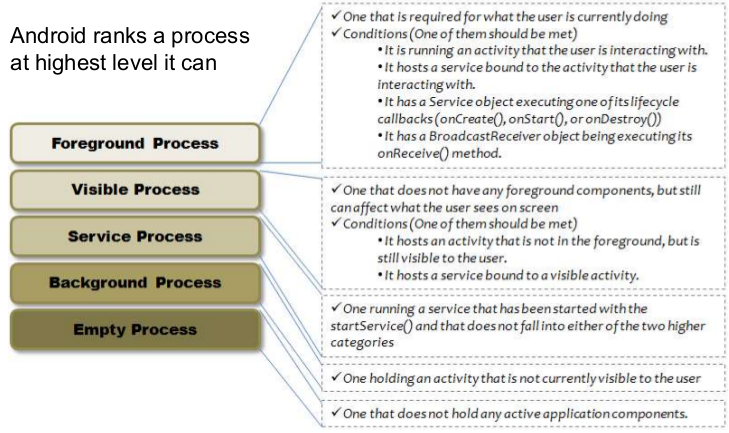
\includegraphics[width=0.24\textwidth]{figures/processImportance.png}

\end{breakbox}

\begin{breakbox}
\boxtitle{UI Thread}

By default all components are instantiated i the main thread of the
specified process. \textbf{Thus the UI is not thread-safe}, the main
thread should be the only one communicating with the UI and is for this
reason called UI thread.

\end{breakbox}

\columnbreak
\begin{breakbox}
\boxtitle{Looper}

Looper class is used to execute the Messages(\textbf{Runnables}) in a
queue. To prepare the Looper use prepare()method. Next, you can use
loop() method to create a message loop in the current thread.

You can also use Looper to check if current thread is the UI thread:

\begin{lstlisting}
If(Looper.myLooper() == Looper.getMainLooper())
\end{lstlisting}
\end{breakbox}
